% !TeX spellcheck = en_GB

\documentclass[a4paper,12pt]{article}


\usepackage{alltt, fancyvrb, url}
\usepackage{graphicx}
\usepackage{subfigure}
\usepackage{wrapfig}
\usepackage{algorithmic}
\usepackage[utf8]{inputenc}
\usepackage{fontenc}
\usepackage{amsmath,stmaryrd,mathtools,algorithm}
\usepackage{amssymb}
\usepackage{longtable}
\usepackage{multirow}
\usepackage{setspace}
\usepackage{todonotes}
\usepackage{csquotes}
\usepackage[margin=1.05in]{geometry}
\usepackage{todonotes}

% Remove option to use English naming
\usepackage[colorlinks,
	linkcolor={red!70!black},
	citecolor={blue!80!black},
	urlcolor={blue!50!black}]{hyperref}
\usepackage[nameinlink]{cleveref}

\usepackage{xcolor}
\usepackage{textcomp}
\usepackage{listings}


\definecolor{myPink}  {rgb}{0.67, 0.05, 0.57} % keywords
\definecolor{myRed}   {rgb}{0.87, 0.20, 0.00} % strings
\definecolor{myGreen} {rgb}{0.00, 0.47, 0.00} % comments
\definecolor{myBrown} {rgb}{0.39, 0.22, 0.13} % brown

\lstdefinestyle{Xcode} {
	language        = C,
	basicstyle      = \footnotesize\ttfamily,
	identifierstyle = \color{black},
	commentstyle    = \color{myGreen},
	keywordstyle    = \color{myPink},
	stringstyle     = \color{myRed},
	directivestyle  = \color{myBrown},
	extendedchars   = true,
	tabsize         = 4,
	showspaces      = false,
	showstringspaces = false,
	breakautoindent = true,
	flexiblecolumns = true,
	keepspaces      = true,
	stepnumber      = 1,
	xleftmargin     = 0pt,
	numbers=left
}

\lstset{
	style=Xcode,
	%caption=lstname,
	breaklines=false,
	frame=single
}

\title{Data visualization -- Process Book\\\textbf{Work in progress}}
\setcounter{tocdepth}{3}
\setcounter{secnumdepth}{3}
 
\author{Mattia Martinelli \and Niccolo Sacchi \and Dario Pavllo}
\date{} %\today

\begin{document}
\pagenumbering{arabic}
\maketitle
\todo[inline]{add table of contents?}
\section{Introduction}
\label{sec:introduction}
Buying from huge e-commerce websites such as \emph{Amazon} has many advantages, but paradoxically, users are often confused by the vast variety of products that are offered. Users may have a rough idea about the characteristics of the product they want to buy, but they often undergo the same process of comparing similar products. We aim to remove this redundancy and aid them in their purchases, suggesting the best or most popular products that correspond to their search. For instance, comparing smartphones or laptops may be difficult due to the wide price range and the required technical knowledge. With our platform, customers can easily visualise in a graphical way what products match their needs, and among them, the most popular and favourite ones.

\subsection{Idea and related work}
Amazon's website already offers a sophisticated search system, which allows users to select category, price range and some technical characteristics of the product they want to buy. But would it not be nice to query among similar articles without explicitly providing to the website such features? For instance, product description  \href{https://www.amazon.com/Acer-E5-575-33BM-15-6-Inch-Notebook-Generation/dp/B01K1IO3QW/ref=sr_1_3?s=pc&ie=UTF8&qid=1512207600&sr=1-3&keywords=laptop}{pages} already contain relevant information about related articles, such as \textit{similar items}, \textit{items bought together} and \textit{items that customers buy after viewing this item}. These links suggest alternatives to the customer; however, they only show \textit{neighbouring} offers and not the whole overview of offers. To overcome this limitation, we have decided to develop a graphical and interactive visualization that shows such relations among multiple articles.

If products are showed as a network, as pictured in \Cref{fig:graphNav}, it is clear to see which ones users usually end up buying. Imagine a user who wishes to buy some professional studio headphones and has a rough idea of their characteristics. By querying the graph, he/she can highlight relevant products and follow the highlighted path towards an optimal product. Of course, defining what articles may be \emph{optimal} is not a trivial task; however, if many clients buy the same product after reviewing a set of other products, then it is very likely that the former is more appealing. 

There may also be groups of products in which it is not possible to identify an optimal one, i.e. users are often uncertain in choosing one of them. Each one of these groups represent a cluster of \textit{competing products}.
\todo[inline]{show an example of clique}

\begin{figure}[H]
	\centering{}
	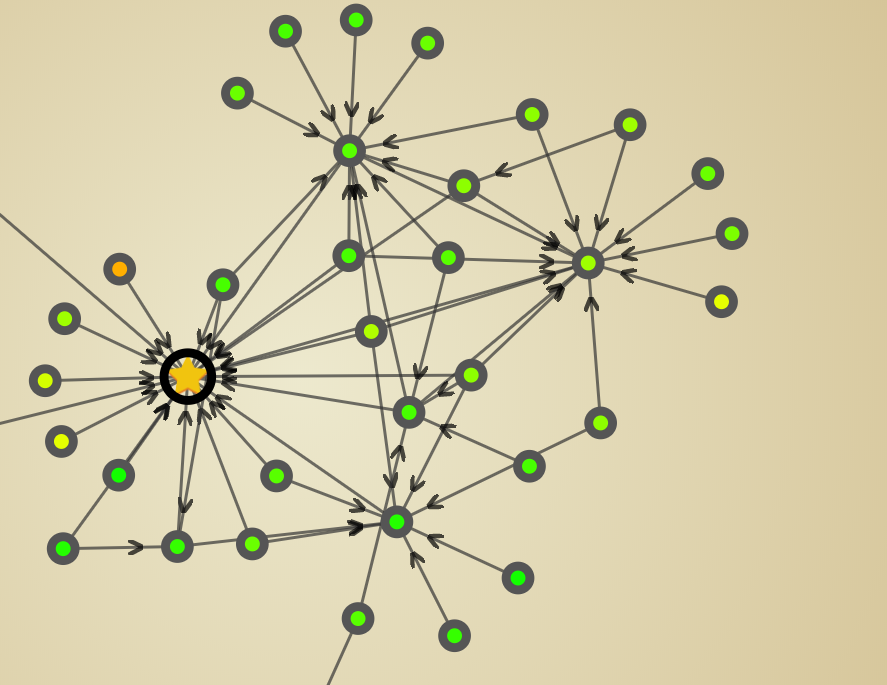
\includegraphics[width=\textwidth]{img/graph_example.png}
	\caption{Subgraph of the \emph{Headphones} category. As can be seen, some nodes (products) are \emph{attractors}, in the sense that users end up buying those after reviewing a large number of other products.}
	\label{fig:graphNav}
\end{figure}
\subsection{Assumptions}
At this point, it could be argued that graph edges provide meaningful relations. We supposed that when users navigate through Amazon's offers, they already have an idea of the product that they want to buy. It can be a technical characteristic, a brand or merely a budget. Our dataset should therefore provide relations contain products that must be similar according to some \textit{human-made} criteria, which would be difficult to extrapolate with a algorithm or a machine learning model.

\subsection{Target audience and use cases}
With our platform we want to address both customers and vendors. Customers may take advantage of previous people's choices to decide what product is worth buying, or to get an idea about alternative items. On the other hand, vendors may explore the visualization to search competitors and see the characteristics of the most popular items in category. \todo{add pictures as example}.

\newpage

\section{Dataset}
\label{sec:dataset}
We have been provided with a dataset of \href{http://jmcauley.ucsd.edu/data/amazon/}{Amazon products} that contains relations among the articles, such as ``bought together'', ``also viewed'', and/or ``buy after viewing''. Such relations have been exploited to create our graph, as explained in \Cref{sec:graph}.
% What about this part?
%These relations will be used for creating a graph that represents competing products with similar characteristics, i.e. products that are viewed together but not bought together. Our assumption is that people interested in a certain product would have visualized and compared similar products prior to buying whichever they consider the best.

\subsection{Description}
The dataset consists of two JSON files:
\begin{itemize}
	\item \textit{metadata}: contains information related to the products, such as their unique ID (\textit{ASIN}), category, description, \textit{sales rank}, brand, price, and  relations with other items. The size of the file is 9.81 GB (uncompressed).
	\item \textit{reviews}: contains ratings and reviews associated to each product, as well as the helpfulness of each review. The size of the file is approximately 87 GB (uncompressed).
\end{itemize}

\subsection{Preprocessing}
Due to the large size of the file, we decided not to exploit the reviews. We created a single dataset where, for each product, we extracted average rating, number of reviews, and their \textit{helpfulness} score. These fields have been then merged with \textit{metadata}.
\todo[inline]{explanation on how components are created. It can be put here, or in the graph section. Also explains the graph as been exported in such a way that keeps categories independet}

\section{The graph}
\label{sec:graph}
The dataset has been transformed into a directed graph, where nodes represent products and edges represent \textit{competitions} between products. 
\subsection{Structure}
The graph structure follows precise rules. An edge from product A to product B is added if clients \textbf{buy} B after viewing A (\textit{buy after viewing} relation), but such edge is removed if A and B are frequently bought together (\textit{bought together} relation). The former means direct competition, i.e. an article has been preferred over another, while the latter means no competition, i.e. the two articles are complementary (e.g. a cellphone and a cover). In our context, a directed edge from A to B means ``B is preferred over A``, whereas an undirected edge (or, equivalently, two opposite directed edges) means ``A is competing with B''. It is easy to extend this definition to groups of competing products, that is, max-cliques. If some groups are totally interconnected, we can assume that they are in direct competition and that one is not necessarily better than the other. 

In previous experiments, we tried to build the graph by adding edges between products that are viewed together (\textit{also viewed} relation). This relation does not imply that any of the products has been actually bought, and it produces a graph that is too dense to give meaningful results.

\subsection{Insights}
By visually inspecting the graph, it is possible to identify some common structures.
\begin{itemize}
	\item \textbf{Accumulators:} these are popular products that have many incoming edges.
	\item \textbf{Max-cliques:} groups of products that are totally interconnected. In many cases, these products are also accumulators. Cliques represent products that are in direct competition with each other (and it is not really clear which one ``wins"). Note that these competition relations might even comprehend products of the same brand.
\end{itemize}
\begin{figure}
	\centering{}
	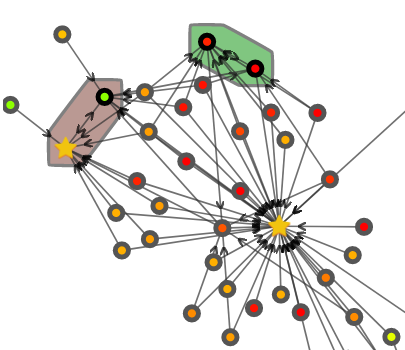
\includegraphics[width=0.45\textwidth]{img/insights.png}
	\caption{Portion of the graph of a category. The stars represent accumulators, whereas the groups represent cliques.}
	\label{fig:insights}
\end{figure}
We have inspected such figures to insure that they have a meaningful representation, both manually and by means of specific algorithms. We could confirm that accumulators represent popular products and cliques represent products with very similar characteristics.

\section{Sketch design}
\label{sec:sketch}
The section shows our original design idea and how we have devised the visualization. Simple sketches that we have made prior to start the implementation are also proposed.

\subsection{Preface}
Before visualizing the graph, the user must choose a category.
We decided to keep categories independent for the following reasons:
\begin{itemize}
	\item The visualization is cleaner and faster to process. If items of multiple categories were mixed, the visualization would result slower and more difficult to interpret.
	\item Items in cliques usually belong only to a single category. Indeed, it would be meaningless to cluster similar products if such products belong to different categories.
	\item We show products that are most popular within only a single category.
\end{itemize}

\subsection{Navigation process}

\begin{figure}[H]
	\centering{}
	
\includegraphics[width=\textwidth]{img/amazon.png}
	\caption{Introductory screen of the webpage.}
	\label{fig:amazon}
\end{figure}
In summary, the visualization guides the user from their idea of product to the final result. In particular, the process should be as follows:

\begin{enumerate}
	\item As an introduction, the user is presented with a brief and intuitive description of the project (\Cref{fig:amazon}). Then, a quick tutorial will be also included to explain how to use the platform.
	\item The user is presented with a selector that navigates through the Amazon category tree (\Cref{fig:category}), and allows him/her to select a category (e.g. headphones, mobile phones, laptops, etc.). It will also be possible to search for a category according to some keywords.
	\begin{figure}[H]
		\centering{}
		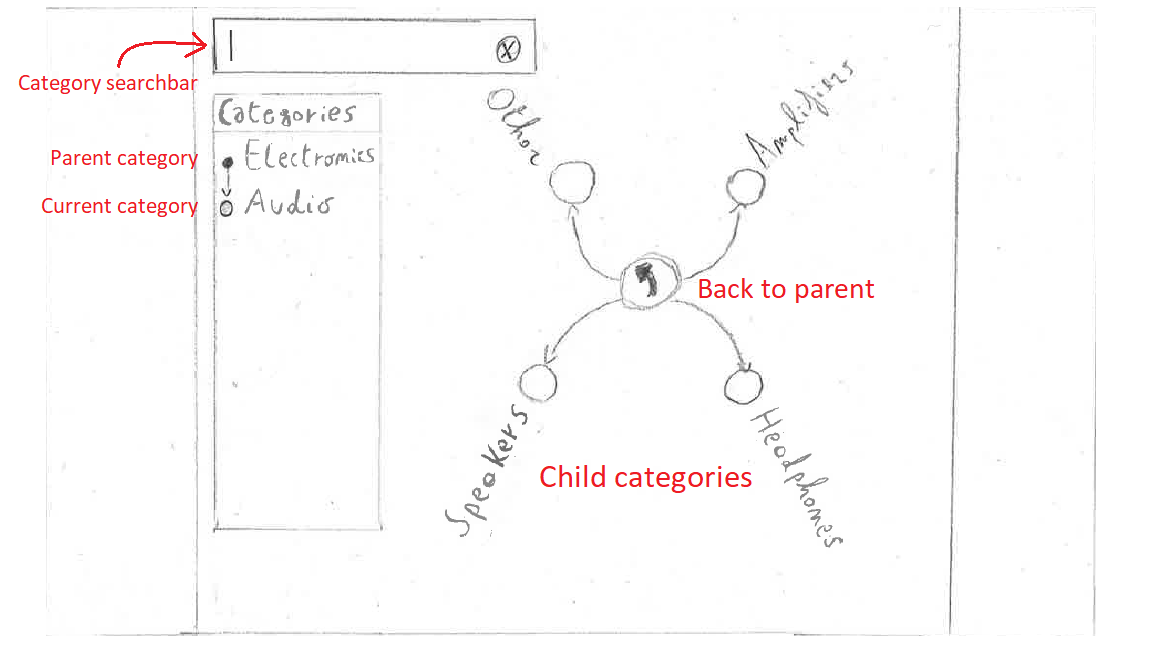
\includegraphics[width=\textwidth]{img/categories.png}
		\caption{Category navigation.}
		\label{fig:category}
	\end{figure}
	\item Once a category is selected, the graph view appears (\Cref{fig:graph}). Initially, the full graph is shown, so that the user can get a sense of its topology (sparseness, attractors, cliques, etc.).
		\begin{figure}[H]
		\centering{}
		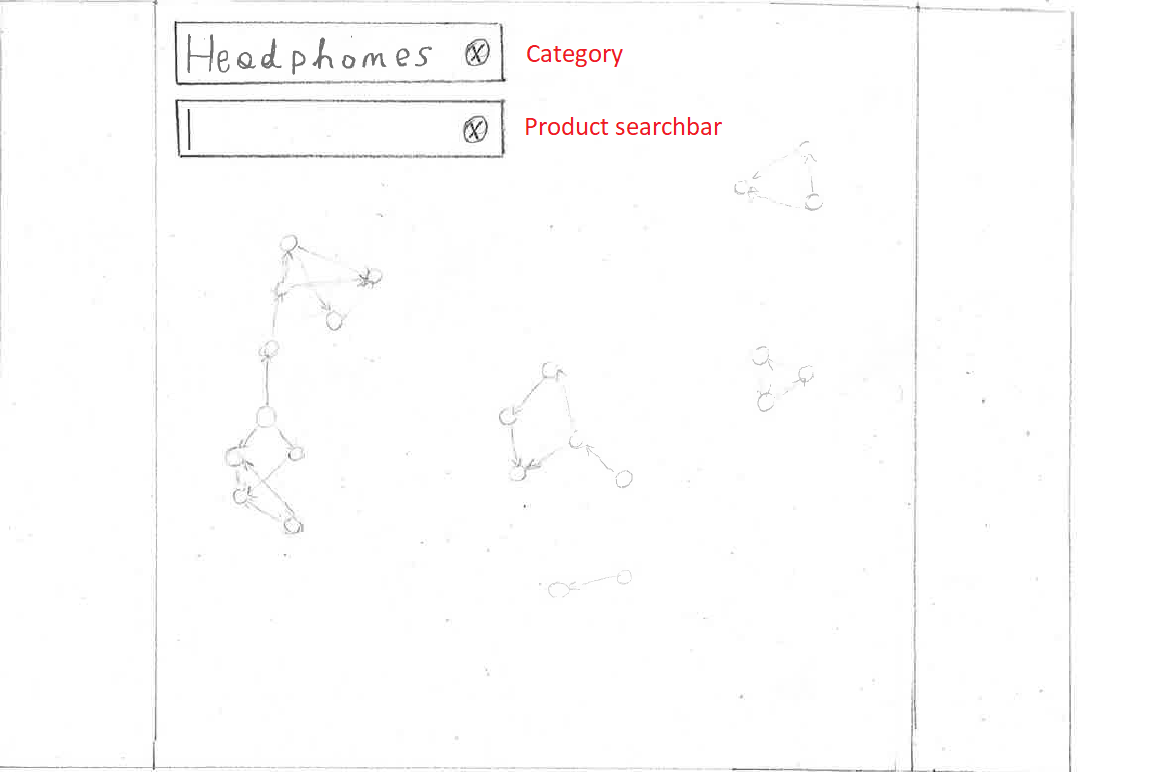
\includegraphics[width=\textwidth]{img/graph.png}
		\caption{The whole graph is shown when a category is selected.}
		\label{fig:graph}
	\end{figure}
	\item The user can query a few keywords and set a price range, which will cause the graph to highlight only relevant parts and collapse the rest (\Cref{fig:wireless}). At this point, the user can inspect the paths between products, as well as the \emph{attractors}. The visualization will also provide some recommendations (automatic paths) and display the characteristics of the products, along with their differences.
		\begin{figure}[H]
		\centering{}
		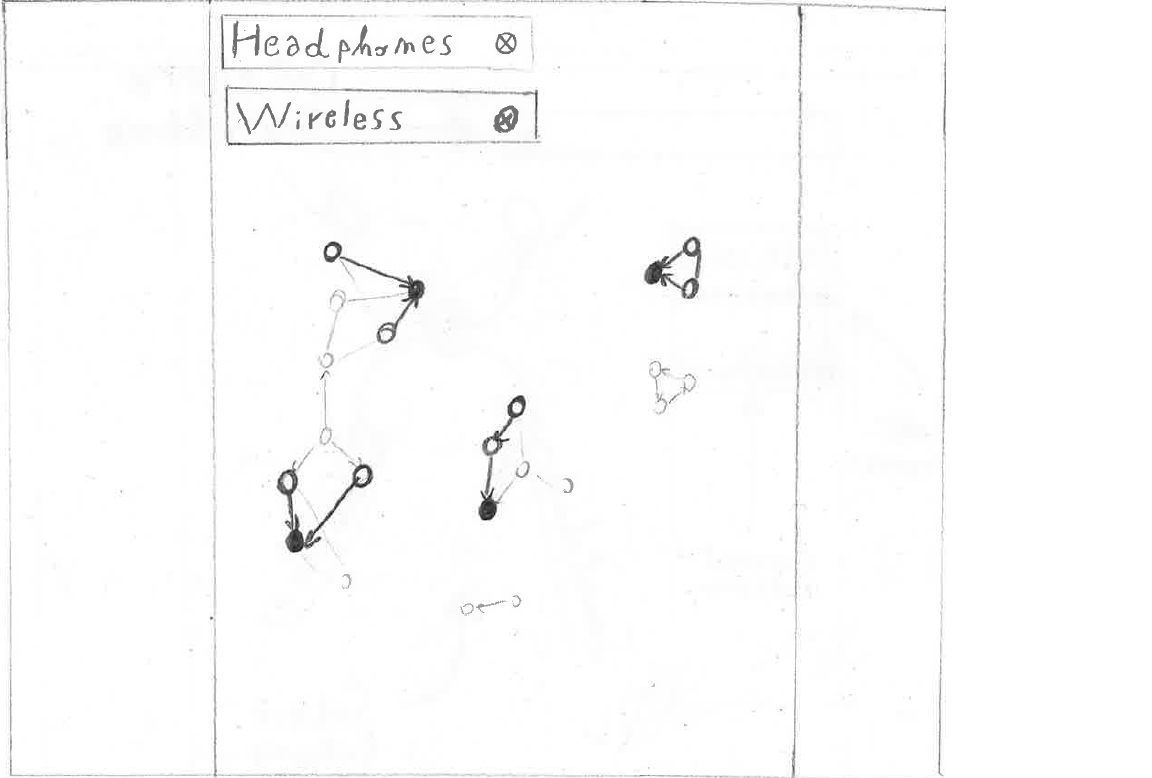
\includegraphics[width=\textwidth]{img/wireless.png}
		\caption{Example of products filtered according to keyword.}
		\label{fig:wireless}
	\end{figure}
	\item The visualization provides some recommendations, showing title, picture and a brief summary of their characteristics (\Cref{fig:best}). Such recommendations are \textit{attractors}, that is, nodes with the highest incoming edges. Therefore, they are considered the most popular products in category.
	\begin{figure}[H]
	\centering{}
	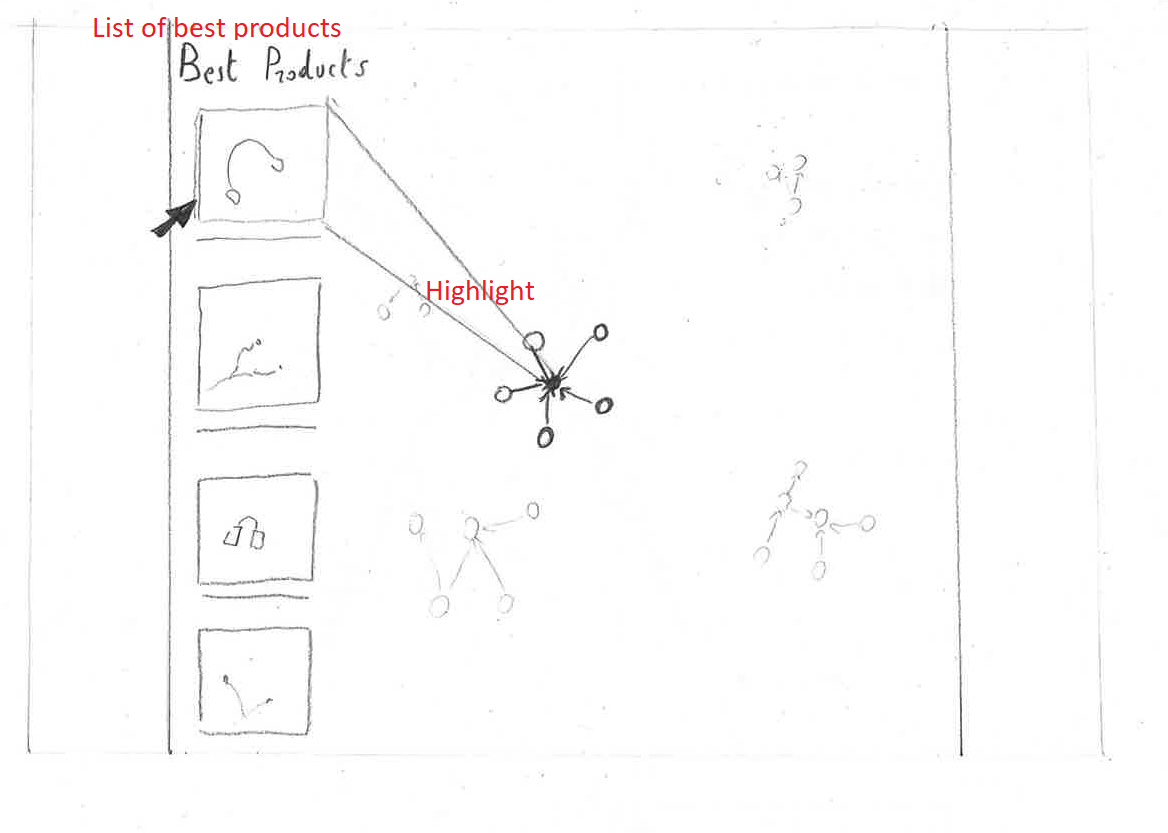
\includegraphics[width=\textwidth]{img/best.png}
	\caption{Best products are directly shown to users, but they are also highlighted on the graph.}
	\label{fig:best}
\end{figure}
\end{enumerate}

\section{Implementation}


\subsection{Graph algorithm}
\todo[inline]{please Dario help me}

\subsection{Visualization}
The graph must show to users the most relevant products in an intuitive manner. As a crucial requirement, users should find the information of interest "at first glance", without need to interpret the graph. However, making intuitive a graph is not a simple task. In order to achieve the goal we undertook the following steps:
\begin{enumerate}
	\item \textit{Product Graph choice}. We opted for \href{http://bl.ocks.org/GerHobbelt/3071239}{this} collapsible graph which would allow to "hide" all the competing products in one node and expand it only if the user is really interested in analazying them. 

	\item \textit{Product Graph: code cleaning and improvements}. After diving in the code of that example we realized how many were the problems. Changes were needed in order to satisfy all our requirements since the code was not versatile, inefficient (e.g. the graph was initially recomputed every time a node was collapsed/expanded) and it used d3 v2. We needed both a structure that would allow to easily update the graph (exclude/include nodes) and code easy to maintain (so to apport changes easily). Therefore, we restructured most of the code implementing classes (which improved versatility and manageability), removed a couple of features we did not need and improved the efficiency. Then, we converted the code to d3 v4 (non easy task, we discovered d3 v4 is not much retro-compatible) so to obtain something more versatile and efficient. However, we understood that collapsing and expanding a node would imply non trivial changes to our graph algorithms, e.g. finding and highlighting the path to the best product (depending whether a clique is expanded or not the path to be highlighted changes). Moreover, the cliques are small and few and the time spent in implementing ad-hoc graph algorithms to keep collapsible nodes would not be worth much. So we decided to indicate the cliques with polygon hulls (d3.polygonHull) so to keep indicating the them. Finally we added arrows instead of edges, since the direction of the edge is of major importance in our algorithm.  We ended up with a graph where cliques were well distinguishable but it was still not very intuitive as the user wouldn't see products but only dots connected by edges.

	\item \textit{Product Graph: add interactivity}. Once we display all the products of a category as a graph the next step is to choose an intuitive and easy way to explore and/or select only the parts of the graph in which the user is interested. To accomplish the task we added several features.
		\begin{itemize}
			\item When the user mouseover a node, we show photo, link, and other imformation of the product. Moreover we also  highlight the path to the best product, i.e. a star.
			\item We add a search box to filter the graph using a keyword. This searchbox has autocompletion and it suggests the words that have been extracted from the title of the products so that the user does not end up in selecting an empty graph. In particular, we show not only the products related to that keyword but also all the reachable nodes and the direct parents. In this way we both show all the better products and also the fan-in of the filtered products (note: the fan in is the metric we choose for selecting the best product between competing products, i.e. products belonging to the same clique).
			\item We show in an hamburger menu the list of computed best products of the whole graph. Those products are also indicated by stars on the graph so to show that the best products are the ones with many incoming edges.
			\item We used the color to encode the price. In particular we sort all the product prices, split them in six bins and then give a color to each bin. However, outliers, e.g. products with very high prices, end up in having the same color of products with a very different price. To reduce this problem we add a brushable price bar with which the user can focus on the products whose price belong to a specific interval. Notice that we keep all the products since filtering out the products that does not belong to the interval could also filter out the best products, e.g. the user could select the price interval 50€-70€ while the best product costs 40€. 
		\begin{itemize}

	\item \textit{Category Graph}. To allow the user select a category and see as well the number of products, we implement an expandible radial tree accompanied by the list (on the left) of explored categories. 

	\item \textit{Packaging}. Once we have both the product graph and the category graph there is the more important setp: package them in good looking and easy usable way.
\end{enumerate}

\section{Conclusion}
We now conclude the process book self-evaluating our visualization and proposing further improvements.
\subsection{Evaluation}
\todo[inline]{judge our visualization, what to we learn from data and how does it answer the problem}
\subsection{Further improvements}
\todo[inline]{Perfomance and visualization improvement}

\newpage

\setcounter{secnumdepth}{0} %% no numbering
\section{Additional notes}
\subsection{Peer evaluation}
\begin{itemize}
	\item Preparation: we have always shared all the necessary information by means of online communication channels, and we have never let a team member to be not up-to-date with the development status.
	\item Contribution : every member of the team has put great effort to keep a constant and uniform pace during the development of the project.
	\item Respect: we have always encouraged different ideas, even though sometimes it might have been tough to reach a consensual agreement. 
	\item Flexibility: Overall, no team member has never complained about criticisms or divergences. We have always tried to ensure consensual agreement, and we have never imposed a solution over another (even in case of majority vote).
\end{itemize}

\subsection{Work disclaimer}
In the initial project proposal form, we stated that our Data visualization project was jointed to our Applied data analysis project. Although we have deployed the same dataset in both courses, the goals (and the developments) of the two project have significantly diverged. While in this course we have focused merely on the visualization of the graph, in the other one we have exploited it for a deep analysis (machine learning and statistics). In addition, for this course we needed some different and more suitable preprocessing of the data for the visualization. We therefore apologize, and we deny our original statement.
\end{document}
